\begin{figure}
    \centering
    \usetikzlibrary{arrows, calc, shapes.geometric}

\tikzstyle{new} = [
    rectangle, 
    rounded corners, 
    minimum width=3cm, 
    minimum height=1cm,
    text centered, 
    text width=3cm,
    draw=black, 
    fill=red!30
]
\tikzstyle{old} = [
    rectangle, 
    rounded corners, 
    minimum width=3cm, 
    minimum height=1cm,
    text centered, 
    text width=3cm,
    draw=black, 
    fill=blue!30
]
\tikzstyle{arrow} = [thick,<->,>=stealth]

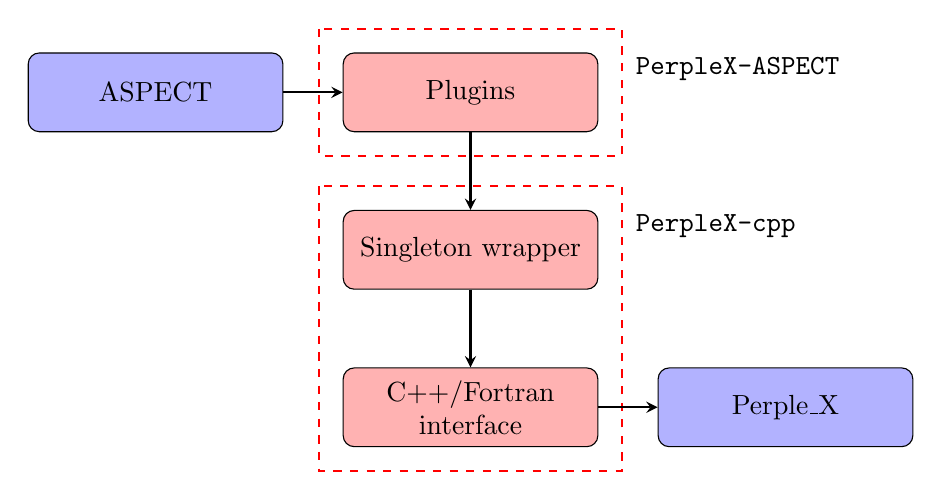
\begin{tikzpicture}[node distance=2cm]
    \node (aspect) [old] {ASPECT};
    \node (plugins) [new, right of=aspect, xshift=2cm] {Plugins};
    \node (singleton) [new, below of=plugins] {Singleton wrapper};
    \node (interface) [new, below of=singleton] {C++/Fortran interface};
    \node (perplex) [old, right of=interface, xshift=2cm] {Perple\_X};
    
    \draw[red, thick, dashed, label=test] 
        ($(plugins.north west)+(-0.3,0.3)$) rectangle 
        ($(plugins.south east)+(0.3,-0.3)$);
    \draw[red, thick, dashed]     
        ($(singleton.north west)+(-0.3,0.3)$) rectangle 
        ($(interface.south east)+(0.3,-0.3)$);
        
    \node (label1) [
        right of=plugins,
        xshift=1.6cm, 
        yshift=0.3cm,
        text width=3cm
    ] {\texttt{PerpleX-ASPECT}};
    \node (label2) [
        right of=singleton, 
        xshift=1.6cm, 
        yshift=0.3cm,
        text width=3cm
    ] {\texttt{PerpleX-cpp}};
    
    \draw [arrow] (aspect) -- (plugins);
    \draw [arrow] (plugins) -- (singleton);
    \draw [arrow] (singleton) -- (interface);
    \draw [arrow] (interface) -- (perplex);
\end{tikzpicture}
    \caption{
        Diagram displaying the flow of data through the program. 
        The red blocks represent the new code and the blue blocks represent the reused code.
        The libraries are denoted with the red dotted lines.
    }
    \label{fig:dataflow}
\end{figure}

The submitted code is split into two libraries, each kept in a separate repository.
The first library, called \texttt{PerpleX-cpp} (\url{http://github.com/cward97/perplex-cpp}), contains the C++/Fortran interface and singleton wrapper that interface with Perple\_X, and consists of both Fortran and C++ code.
The second, called \texttt{PerpleX-ASPECT} (\url{http://github.com/cward97/perplex-aspect}), contains the plugin code that implements the wrapper inside of ASPECT and is written entirely in C++.
The code for both libraries is compiled using CMake.
A diagram displaying the relationship between the repositories as well as Perple\_X and ASPECT is shown in Figure~\ref{fig:dataflow}.
Alongside the source code, a wiki is provided giving useful information about topics such as setting up a development environment on the Hamilton supercomputer, viewing the results in Paraview, and using Docker.

The justification for splitting the code into two repositories is twofold.
Firstly, it ensures that the Perple\_X wrapper code is entirely general and the library can be used outside of ASPECT.
Secondly, it enforces a separation between ASPECT and Perple\_X.
This is potentially valuable if the plugin code were to be integrated upstream into the main ASPECT repository.

Regarding the code licensing, both Perple\_X and ASPECT are licensed under the GNU Public \mbox{Licence} (GPL) version 2.
In order for the submitted code to be compliant with these licences it has been licensed using the more modern GPL version 3.

\subsection{\texttt{PerpleX-cpp}}

Perple\_X consists of a suite of several executables written in Fortran 77.
The executable of interest to this project is MEEMUM which computes the stable phases, and their respective compositions, at a given point in $p$-$T$-$X$ space.

Running MEEMUM is generally straightforward although collating a reasonable set of inputs can sometimes be challenging.
Different versions of Perple\_X sometimes refuse to run with certain input files because of minor changes to the way the files are parsed.
The inputs to the program are: 
(a) a problem definition file containing the bulk composition made by another Perple\_X binary BUILD;
(b) a solution model file;
(c) a Perple\_X option file; and
(d) a thermodynamic database file~\parencite[e.g.][]{holland_internally_1998}.
When the program is run it prompts the user for $p$, $T$ and $X$ values and prints the results to the screen.
The aim of the wrapper is to automate this process providing the $p$, $T$ and $X$ conditions as inputs to a function returning the phase information that would otherwise be printed.
The various input files are untouched and are read when the wrapper is first initialised.

\subsubsection{Original Perple\_X source code}
\label{sec:solution_perplexcpp_orig}

Interacting with the Perple\_X code is a complex task and one of the more difficult of this project.
It is written in Fortran 77 and thus has certain features not encountered in a modern programming language, the most significant for this work being the extensive use it makes of COMMON blocks.
In addition, the tools in Perple\_X are designed exclusively for interactive use.
There is no clear separation between the (command line) user interface and the program logic so there are, for example, random places in the code where the user is polled for input.
This makes it challenging to automate the code without making radical changes to the codebase.

The decision was made to directly include the source code inside the repository rather than either encouraging the user to install Perple\_X themselves or downloading and compiling the latest version\footnote{The latest version of Perple\_X may be downloaded from \url{https://petrol.natur.cuni.cz/~ondro/perplex}.} during the build.
The principal reason for this is reliability. Perple\_X receives frequent breaking updates and there is no easy way to access old versions, so the source code is stored inside the repository in order to ensure that the code does not break unexpectedly.
The version used in the repository at the time of writing is 6.9.0.

When Perple\_X is downloaded it comes with many files that compile to different executables other than MEEMUM as well as lots of thermodynamic database files and various \texttt{README}s.
To avoid \mbox{confusion}, only the necessary source files are included inside the repository.

\subsubsection{C++/Fortran interface}

The basic concept behind integrating Fortran code into C++ is very simple. All that is required is a C++ header file declaring the required Fortran functions and variables using the correct symbols (e.g. the function \texttt{foo()} is normally represented with the symbol \texttt{foo\_}) and then the codes can be linked during compilation.
However, actually implementing this is far from straightforward: many of the data types are incompatible, array indexing starts from zero (C++) or one (Fortran), and arrays themselves are alternately row-major order (C++) or column-major order (Fortran).

This problem is compounded in Perple\_X by the sheer number of global variables, both constant \texttt{PARAMETER}s and \texttt{COMMON} blocks that are used by the program.
The source code contains a 400 line file called \texttt{perplex\_parameters.h} that contains the program parameters as well as many frequently used \texttt{COMMON} blocks.
If one were to write a C++ wrapper then this file would need to be converted into a C++ header too.

This was done previously by~\textcite{kaislaniemi_prplxwrap_2015}; the parameter file was rewritten by hand into C++.
\textcite{myhill_perplex_2018} improved upon this by writing a Python script that `compiled' the first part of the Fortran parameter file into a C++ header although the latter half still needed manually writing out.

This approach has a number of drawbacks: (a) whenever Perple\_X is upgraded this script must be re-run; (b) the process is complex and hard to debug in case errors occur; and (c) the resulting header file is very hard to read.

In this work, to solve these issues, an additional Fortran file (\texttt{f2c.f}) was created.
Rather than being converted to C++, the parameter file is simply included once in this file, permitting a much simpler C++ header file (\texttt{f2c.h}) to be written.
The new interface provides a small number of getters (e.g. \texttt{get\_endmember\_density()}) and setters (e.g. \texttt{solver\_set\_pressure()}) as well as a largely verbatim copy of the MEEMUM subroutine, only altered to eliminate any calls for user input and split into initialise (called once) and compute (called many times) functions.
Arguments are passed by value (C-like) and only single values are passed (excluding strings), avoiding any complexities involved with arrays.

An additional advantage of this approach is readability.
Having been written in Fortran 77, Perple\_X has a six character limit on its variable names, which can make it very hard to follow what the variables and functions do.
The new interface code was not so restricted, allowing for much more verbose and understandable function names.

A final point about the interface is that, being effectively a duplicate of the original code, the `warm start' functionality of Perple\_X remains active.
This is an obscure feature found in the Perple\_X source code\footnote{The hot start features are implemented in the main \texttt{lpopt0} optimisation routine.} and has unknown performance benefits.
This feature will be ignored for the rest of the document but is recorded here for future reference.

\subsubsection{Singleton wrapper}

Although the basic interface described above is a significant improvement on previous approaches, it is still fairly limited.
Only basic data types are accepted and its use requires interacting with global variables, something that is considered poor software development practice.

Our solution to both these problems is the creation of a \texttt{Wrapper} class.
The class presents \mbox{initialise} and compute methods to the user and hides the details of interfacing with the Fortran \mbox{completely}.
\mbox{Additionally}, it permits the use of more complex data types, such as \texttt{std::vector} and \texttt{std::string}, that are in common use in ASPECT.
An object-oriented solution was chosen because Perple\_X consists of both functions and data, making it a suitable candidate for encapsulation into a class.

The class also implements the \textit{singleton pattern}; that is, only a single instance of the class may ever exist.
This approach was taken in order to prevent concurrent accesses to the global Perple\_X data structures that would otherwise occur if multiple objects existed all accessing the same state.

Having been designed as an interactive program, Perple\_X prints a lot of information to the screen whenever MEEMUM is executed.
Whilst appropriate for use as the main program, it becomes problematic inside the wrapper because it obscures other useful output from the rest of the program.
This is a particular issue if it is called frequently and on multiple processors as the output quickly becomes unreadable.
To avoid this problem, the standard output stream is disabled during the calculations and re-enabled when they are completed.
This fixes the stated problem but introduces another issue. 
Because Perple\_X does not write its error messages to the standard error output stream but instead to standard output, which is disabled, any error messages from Perple\_X will be hidden and the program may crash without \mbox{warning}.
In order to permit the re-enabling of console output in these cases, an \texttt{ALLOW\_PERPLEX\_OUTPUT} compiler flag is introduced, although it is disabled by default.

\begin{figure}[htb]
    \centering
    \usetikzlibrary{arrows, shapes.geometric}

\tikzstyle{startstop} = [rectangle, rounded corners, minimum width=3cm, minimum height=1cm,text centered, draw=black, fill=red!30]
\tikzstyle{io} = [trapezium, trapezium left angle=70, trapezium right angle=110, minimum width=3cm, minimum height=1cm, text centered, draw=black, fill=blue!30]
\tikzstyle{process} = [rectangle, minimum width=3cm, minimum height=1cm, text centered, text width=3cm, draw=black, fill=orange!30]
\tikzstyle{decision} = [diamond, minimum width=3cm, minimum height=1cm, text centered, draw=black, fill=green!30]
\tikzstyle{arrow} = [thick,->,>=stealth]

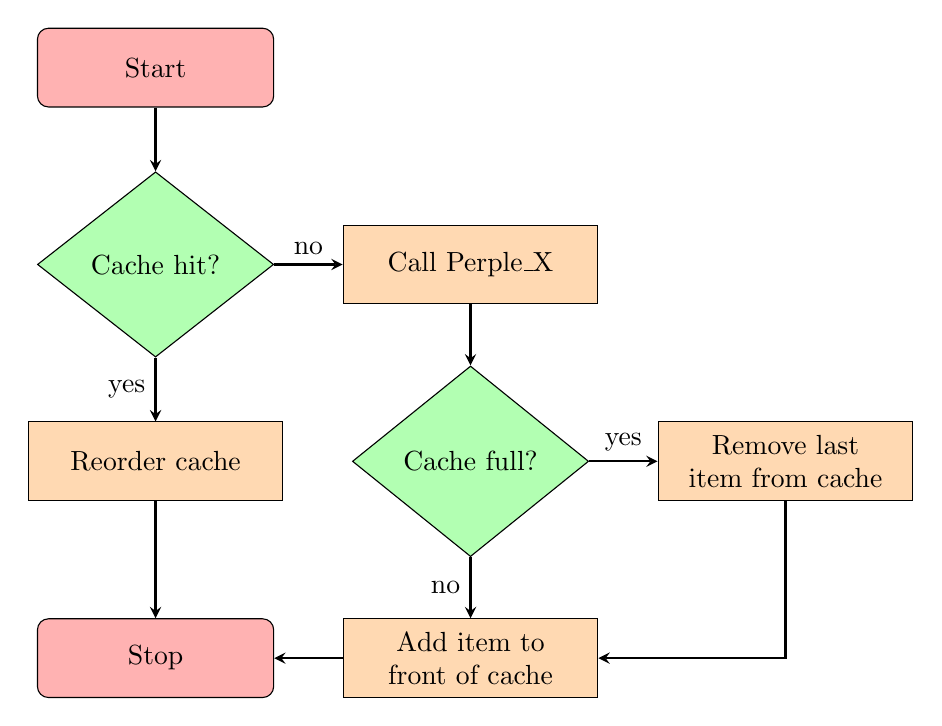
\begin{tikzpicture}[node distance=2cm]
    \node (start) [startstop] {Start};
    \node (dec1) [decision, below of=start, yshift=-0.5cm] {Cache hit?};
    \node (pro1a) [process, right of=dec1, xshift=2cm] {Call Perple\_X};
    \node (pro1b) [process, below of=dec1, yshift=-0.5cm] {Reorder cache};
    \node (dec2) [decision, below of=pro1a, yshift=-0.5cm] {Cache full?};
    \node (pro2a) [process, right of=dec2, xshift=2cm] {Remove last item from cache};
    \node (pro2b) [process, below of=dec2, yshift=-0.5cm] {Add item to front of cache};
    \node (stop) [startstop, below of=pro1b, yshift=-0.5cm] {Stop};
    
    \draw [arrow] (start) -- (dec1);
    \draw [arrow] (dec1) -- node[anchor=south] {no} (pro1a);
    \draw [arrow] (dec1) -- node[anchor=east] {yes} (pro1b);
    \draw [arrow] (pro1a) -- (dec2);
    \draw [arrow] (dec2) -- node[anchor=south] {yes} (pro2a);
    \draw [arrow] (dec2) -- node[anchor=east] {no} (pro2b);
    \draw [arrow] (pro2a) |- (pro2b);
    \draw [arrow] (pro1b) -- (stop);
    \draw [arrow] (pro2b) -- (stop);
\end{tikzpicture}
    \caption{Flowchart showing the decision process for the least recently used (LRU) cache used by the \texttt{Wrapper} class.}
    \label{fig:cache_flowchart}
\end{figure}

During the project, it was noticed that many computations were being done with identical or almost identical inputs. 
It therefore made sense to store the most frequently used results and use them if \mbox{subsequent} inputs are sufficiently similar.
A cache was implemented using a least recently used (LRU) eviction policy.
In other words, it only stores the most recently used results, and results that have not been needed for a while are removed to save memory and must be recomputed if needed again.
A flowchart detailing the decision process for an LRU cache is shown in Figure~\ref{fig:cache_flowchart}.
Cache accesses are defined as being \textit{hits}, where a matching result is found and returned, and \textit{misses}, where no match is found.
The \textit{hit rate} is simply the number of cache hits divided by the total number of cache requests.
In this work, a cache hit is considered to have occurred when each of the submitted $p$-$T$-$X$ conditions varies by less than a specified relative tolerance, normally on the order of \num{1e-3}.

\subsubsection{Testing}

The library is tested using the Google C++ unit testing framework Google Test.
For the C++/Fortran interface and singleton wrapper class, the tests consist largely of a direct comparison between the results of the function calls and previously collected Perple\_X output for a quick-to-run sample data set.
More traditional unit tests testing the behaviour of individual functions have also been written for the cache implementation.

\subsubsection{Parallelism}

Perple\_X is not designed for parallel execution and as such the library is not thread-safe. 
However, there are only a few methods that are exposed to the user so it would be straightforward to add locks to them, making them thread-safe.
In contrast, the code is entirely suitable for parallelism in a distributed memory environment (i.e. MPI) because the global state is still local to each processor.
MPI is the primary parallelisation method used within ASPECT and so thread-safety was not considered a necessary feature of the library.

\subsection{\texttt{PerpleX-ASPECT}}

The Perple\_X wrapper code was integrated into ASPECT using its powerful \textit{plugin} system.
Within ASPECT, plugins are pieces of code that fulfil a particular piece of functionality; for example, declaring the initial temperature profile.

When it comes to integrating the new plugins with ASPECT, there are two main options:
forking and modifying the main ASPECT repository, or creating another repository and compiling it into a shared library so that it can be linked to ASPECT at runtime.
The latter was chosen for the following reasons: 
(a) updating ASPECT does not require either rebasing or merging the git repositories;
(b) not having the new code mixed in with the original code makes things clearer; and 
(c) the code is rather specialist and may not ultimately be added to the ASPECT codebase.

The plugins expose to the user a set of options that may be included in the parameter file that is submitted to ASPECT.
Given the small number of source files that are written, no automatic method of generating the documentation has been written and we recommend reading the source code for \mbox{parameter} details. 
Some example parameter files are included in the \texttt{cookbooks} directory in the repository providing examples of how to use the plugins.

\subsubsection{Particle property plugin}

Within ASPECT there exist several plugins related to tracking particles, sometimes known as tracers, around the simulation.
In this work, an additional \textit{particle property} plugin was written that returns phase information from Perple\_X using the pressure, temperature, and (at least initially) the bulk composition given in the problem definition file.

The basic idea of particles in a geodynamical simulation is that they are point objects passively advected around the medium with the velocity field.
They store a set of properties that are updated at specified time steps using the state of the different fields present at their current position.

It is easy to control the performance of particles inside of a simulation because both the increment between updates and the number of particles are options that may be specified in the parameter file.
This is particularly useful for investigations with Perple\_X because each evaluation can take a considerable amount of time to complete.
An additional benefit of using particles is that they do not, unless desired, interfere with the rest of the simulation.
This is an advantage over the material model plugin discussed next which restricts the code to using a single material model.
However, it is important to note that performance is poor when dealing with large numbers of particles, as the implementation still requires some optimisation, or when using a highly-adaptive mesh, as load balancing does not take into account the number of particles and instead only considers the number of degrees of freedom that are related to the cell count.

The plugin has been designed to accept many different parameter options permitting access to many of the results reported by Perple\_X and the wrapper code.
Results for any of the possible solution phases, including the melt, are available and properties such as the composition, molar amount and volume fraction may all be specified.
It would be straightforward to extend the list of available properties to include any that are reported as output from MEEMUM.

One particularly noteworthy set of options permitted by the plugin are \texttt{Extract melt} and \texttt{Melt extraction threshold}.
These permit an investigation of fractional melting of the material.
If \texttt{Extract melt} is set to \texttt{true} then whenever the melt volume fraction exceeds the specified \mbox{threshold}, typically around 5\%, then the melt is removed from the simulation, altering the bulk composition accordingly.
If this option is enabled, then the plugin will automatically report on the amount of moles and composition of both the melt that is extracted and the melt that is present within the bulk material.
Relative properties such as the volume fraction of the extracted melt are not tracked because they are non-physical quantities.

\subsubsection{Material model plugin}

Despite its many benefits in performance and simplicity, the particle property plugin is incompatible with a study of two-phase flow which is desirable for a realistic model of melt behaviour.
This is because two-phase flow requires that the composition of the melt be advected separately to the composition of the residue, one being solid and the other a fluid.
In ASPECT, particles can be set to either advect with the melt field \textit{or} with the solid material, but not both.
In this work we avoided this problem by pivoting to a compositional field-based approach and implementing a new \textit{material model} plugin.

\vspace{5mm}

Compositional fields are extra fields in ASPECT whose motion is solved by one of the four \mbox{equations} used in ASPECT:

\begin{equation*}
    \frac{\partial c_i}{\partial t} + \mathbf{u} \cdot \nabla c_i = q_i.
\end{equation*}

The compositional fields $c_i$ are advected with the flow velocity $\mathbf{u}$ with an optional \textit{reaction term} $q_i$ to handle reactions between the fields. Although similar to particles in that they are advected with a velocity field, compositional fields are able to be advected with the melt velocity field as well as with the usual, solid velocity field which is what makes two-phase flow possible. 

For our work, several compositional fields were introduced, each representing a given chemical \mbox{component} for either the melt or the residue, as well as an additional compositional field called the \textit{porosity} that must be included for models with melt transport and represents the volume fraction of the melt. 
In our investigations, given that the Perple\_X model we were using specified four chemical components, we used nine compositional fields: four for the melt, four for the residue, and the porosity.

An unfortunate downside to this approach is that the parameter files become significantly more \mbox{complex} as the compositional fields must be specified by name and must correspond exactly to the compounds specified in the Perple\_X problem file.
Examples demonstrating the correct usage of the plugin may be found inside the repository.

\vspace{5mm}

In ASPECT, the material model is responsible for calculating the various coefficients, such as the viscosity, density and specific heat, that are required in order to solve the main equations.
Reactions between compositional fields are controlled by specifying reaction terms (zero by default).
The principal method of any material model plugin is called \texttt{evaluate()} which is called multiple times at every time step to calculate the coefficients.
These coefficients are often evaluated at multiple quadrature points inside of each cell.

The material model plugin that was implemented inherits from the \texttt{melt simple} material model found in the main ASPECT repository.
This choice was made because writing a material model from scratch that implements partial melting was found to be very difficult leading to catastrophic convergence errors.
Instead, the new model simply extends the \texttt{evaluate()} method and overrides the \texttt{melt\_fractions()} method.
In both of these methods, the chemical composition is extracted from ASPECT's compositional fields and passed to the Perple\_X wrapper along with the pressure and \mbox{temperature}.
The result from the calculation is then used to either report on the volume fraction of melt or update the compositional fields.

The decision to use the \texttt{melt simple} model as the base over the very similar \texttt{melt global} model was arbitrary and the submitted code could easily be adapted to inherit from that model instead.

For models with melt migration, the processes of melting and freezing typically occur on a much faster time scale than even the flow of the melt itself.
In order to decouple the two processes the \textit{operator splitting} scheme is used, where for every advection time step, multiple reaction time steps occur.
A consequence of this method is that there are a great many calls to Perple\_X but this is necessary for a realistic model.

Finally, so as to resolve the melt reaction and advection processes with a higher resolution than the solid material, the \texttt{composition threshold} mesh refinement strategy is used to ensure that areas where melt is present are refined to a greater extent.

\subsubsection{Additional plugins}

In addition to the plugins discussed above, \textit{postprocessor} and \textit{initial composition} plugins were also written.
The postprocessor plugin is called \texttt{perplex cache statistics} and it permits analysis of the cache in the Perple\_X wrapper.
The initial composition plugin is called \texttt{perplex composition} and it makes sure that the compositional fields representing the melt and residue compositions (for two-phase flow) are initialised correctly using the initial Perple\_X data file for the bulk composition.

\subsubsection{Testing}

Unit testing is difficult to do in ASPECT, as evidenced by the fact that very few unit tests actually exist in the main repository, due to the fact that plugins are tightly integrated with the rest of the simulation.
Most plugins inherit from the \texttt{SimulatorAccess} class in order to access information from the rest of the simulation such as time step number or to interact with other plugins.
Such tight coupling makes unit testing of single pieces of functionality practically impossible.

Instead of using unit tests, ASPECT relies upon \textit{benchmarks} for evidence of its accuracy.
These involve running simulations with a known answer, for example the temperature change over a phase transition, and verifying that the ASPECT code converges to the correct answer.
The decision was made to not include any benchmarks with the code because they require detailed domain-specific knowledge and were impractical to include given the time constraints of the project.

The other form of testing used in ASPECT is much less informative.
The \texttt{tests} directory in the repository contains hundreds of parameter files, each very quick to run and only a few time steps in duration.
Also stored are the output files produced when running each of the parameter files.
This allows for a very simple test to verify that the code runs as expected by simply rerunning the model setups and checking that the outputs have not changed.
In ASPECT the process has been cleverly automated and relies on utilities such as \texttt{diff} to determine a pass or fail.
The implementation of this is rather complicated so in our work we rely upon making manual comparisons of the outputs.
A few simple tests of this nature are included in our repository.
